% \begin{wrapfigure}{l}{0.2\textwidth}
%   \begin{center}
%   \vspace{-0.02in}
%     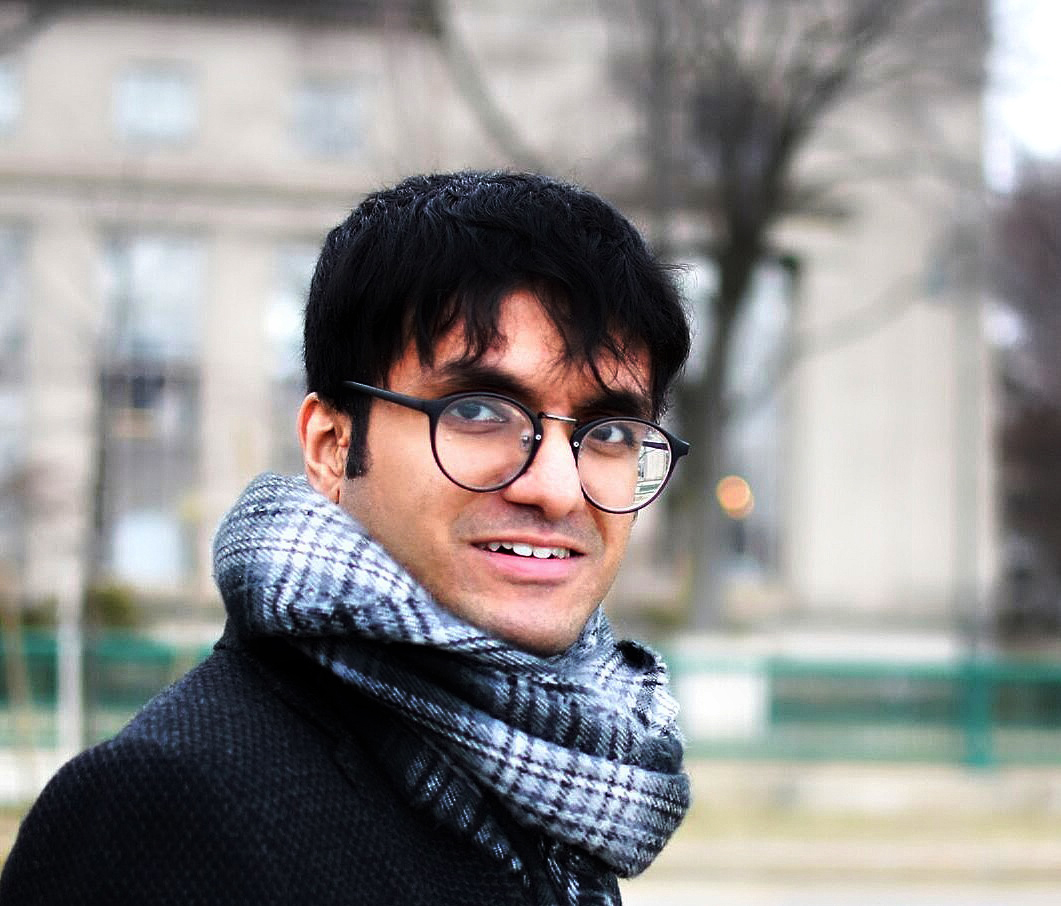
\includegraphics[width=0.19\textwidth]{figures/biography/rahul_shome.jpeg}
%   \hspace{-0.02in}
%   \vspace{-0.02in}
%   \end{center}
% \end{wrapfigure}
% \noindent\textbf{Rahul Shome} is pursuing his Ph.D. in Computer
% Science at Rutgers University, and working with Prof. Kostas Bekris at
% the PRACSYS Lab. His research interests include multi-robot motion
% planning, manipulation planning, and problems in rearrangement task
% planning.  
% \\

% \begin{wrapfigure}{l}{0.2\textwidth}
%   \begin{center}
%   \vspace{-0.02in}
%     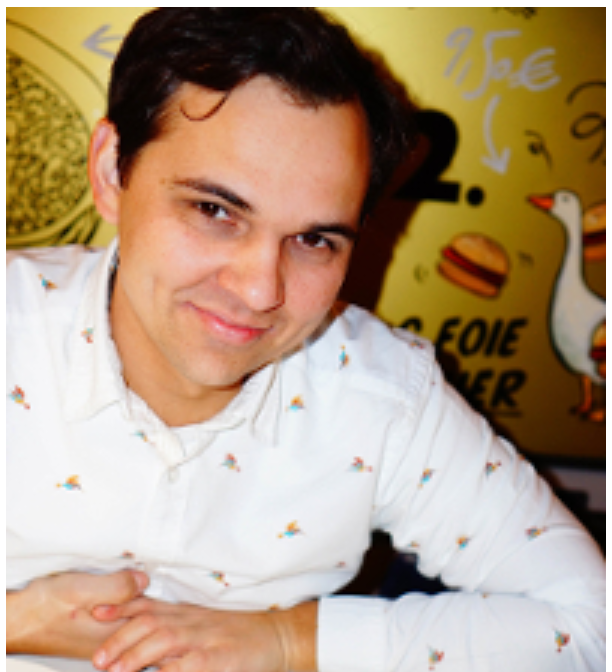
\includegraphics[width=0.19\textwidth]{figures/biography/kiril_solovey.PNG}
%   \hspace{-0.02in}
%   \vspace{-0.02in}
%   \end{center}
% \end{wrapfigure}
% \noindent\textbf{Kiril Solovey} is a Postdoctoral Scholar at the Autonomous Systems Lab, Department of Aeronautics and Astronautics, Stanford University, hosted by Prof. Marco Pavone. His research focuses on algorithmic aspects of robotics. He is particularly interested in the design and analysis of techniques for robot motion planning, multi-robot systems, and autonomous mobility-on-demand. He is supported by the Fulbright Scholars Program. Prior to Stanford, He was a Ph.D. student at Tel Aviv University working with Prof. Dan Halperin in the Computational Geometry Lab. He was supported by the Clore Israel Foundation.\\

% \begin{wrapfigure}{l}{0.2\textwidth}
%   \begin{center}
%   \vspace{-0.02in}
%     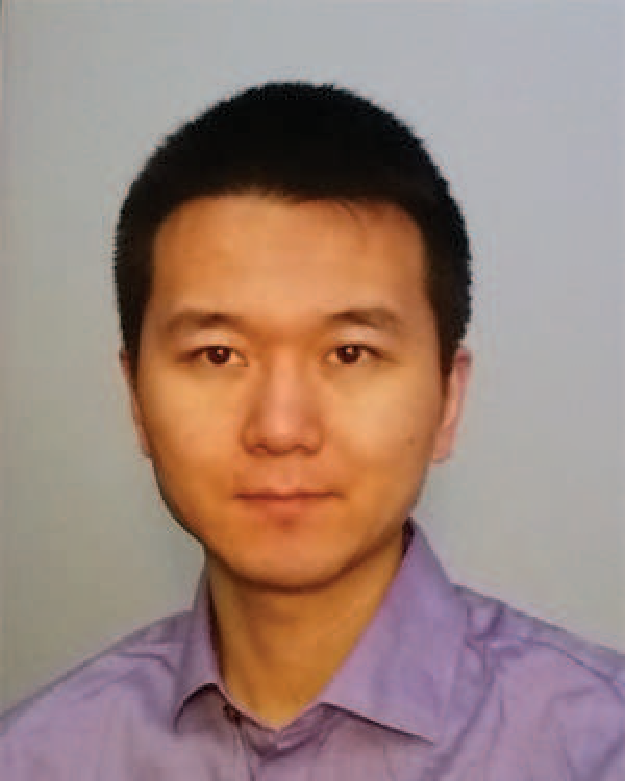
\includegraphics[width=0.19\textwidth]{figures/biography/yu-eps-converted-to.pdf}
%   \hspace{-0.02in}
%   \vspace{-0.02in}
%   \end{center}
% \end{wrapfigure}
% \noindent\textbf{Jingjin Yu} is an Assistant Professor in the Department of Computer Science at Rutgers, the State University of New Jersey. He received his B.S. degree from the University of Science and Technology of China in 1998. He holds M.S. degrees in Chemistry (Univ. Chicago, 2000), Mathematics (Univ. Illinois at Chicago, 2001), and Computer Science (Univ. Illinois at Urbana-Champaign, 2010). He obtained his Ph.D. degree in Electrical and Computer Engineering from the University of Illinois at Urbana-Champaign in 2013, where he briefly stayed as a postdoctoral researcher. He was a postdoctoral researcher at the Massachusetts Institute of Technology from 2013 to 2015 with a joint appointment at Boston University from 2013 to 2014. He is broadly interested in the areas of robotics and control, focusing on issues related to computational complexity and the design of efficient algorithms with provable guarantees. He is a Siebel Scholar and a recipient of the NSF CAREER Award.\\ 
% \\ \\ \\ \\ \\ \\ \\


% \begin{wrapfigure}{l}{0.2\textwidth}
%   \begin{center}
%   \vspace{-0.02in}
%   \noindent 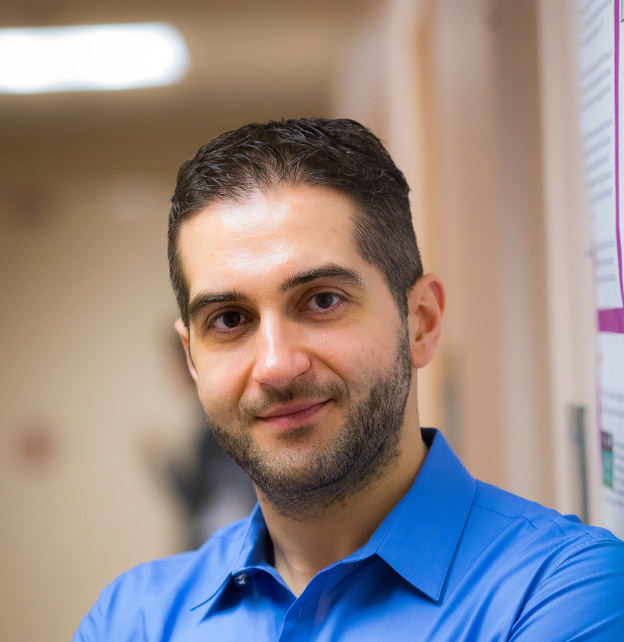
\includegraphics[width=0.19\textwidth]{figures/biography/kostas_bekris.jpg}
%   \hspace{-0.02in}
%   \vspace{-0.02in}
%   \end{center}
% \end{wrapfigure}
% \noindent\textbf{Kostas Bekris} is an Associate Professor in the
% Computer Science department of Rutgers, the State University of New
% Jersey. He received his MS and PhD degrees in Computer Science from
% Rice University in 2004 and 2008 respectively. He was an Assistant
% Professor at the Department of Computer Science and Engineering at the
% University of Nevada, Reno from 2008 to 2012. He is the recipient of a
% NASA Early Career Faculty award and his research has been supported by
% NSF, NASA, DHS and the DoD. His research interests include planning
% and coordination of robots, especially for systems with many degrees
% of freedom and significant dynamics, as well as applications to
% robotic manipulation, planetary exploration, cyber-physical systems
% and physically-realistic virtual agents. \\

% \begin{wrapfigure}{l}{0.2\textwidth}
%   \begin{center}
%   \vspace{-0.02in}
%     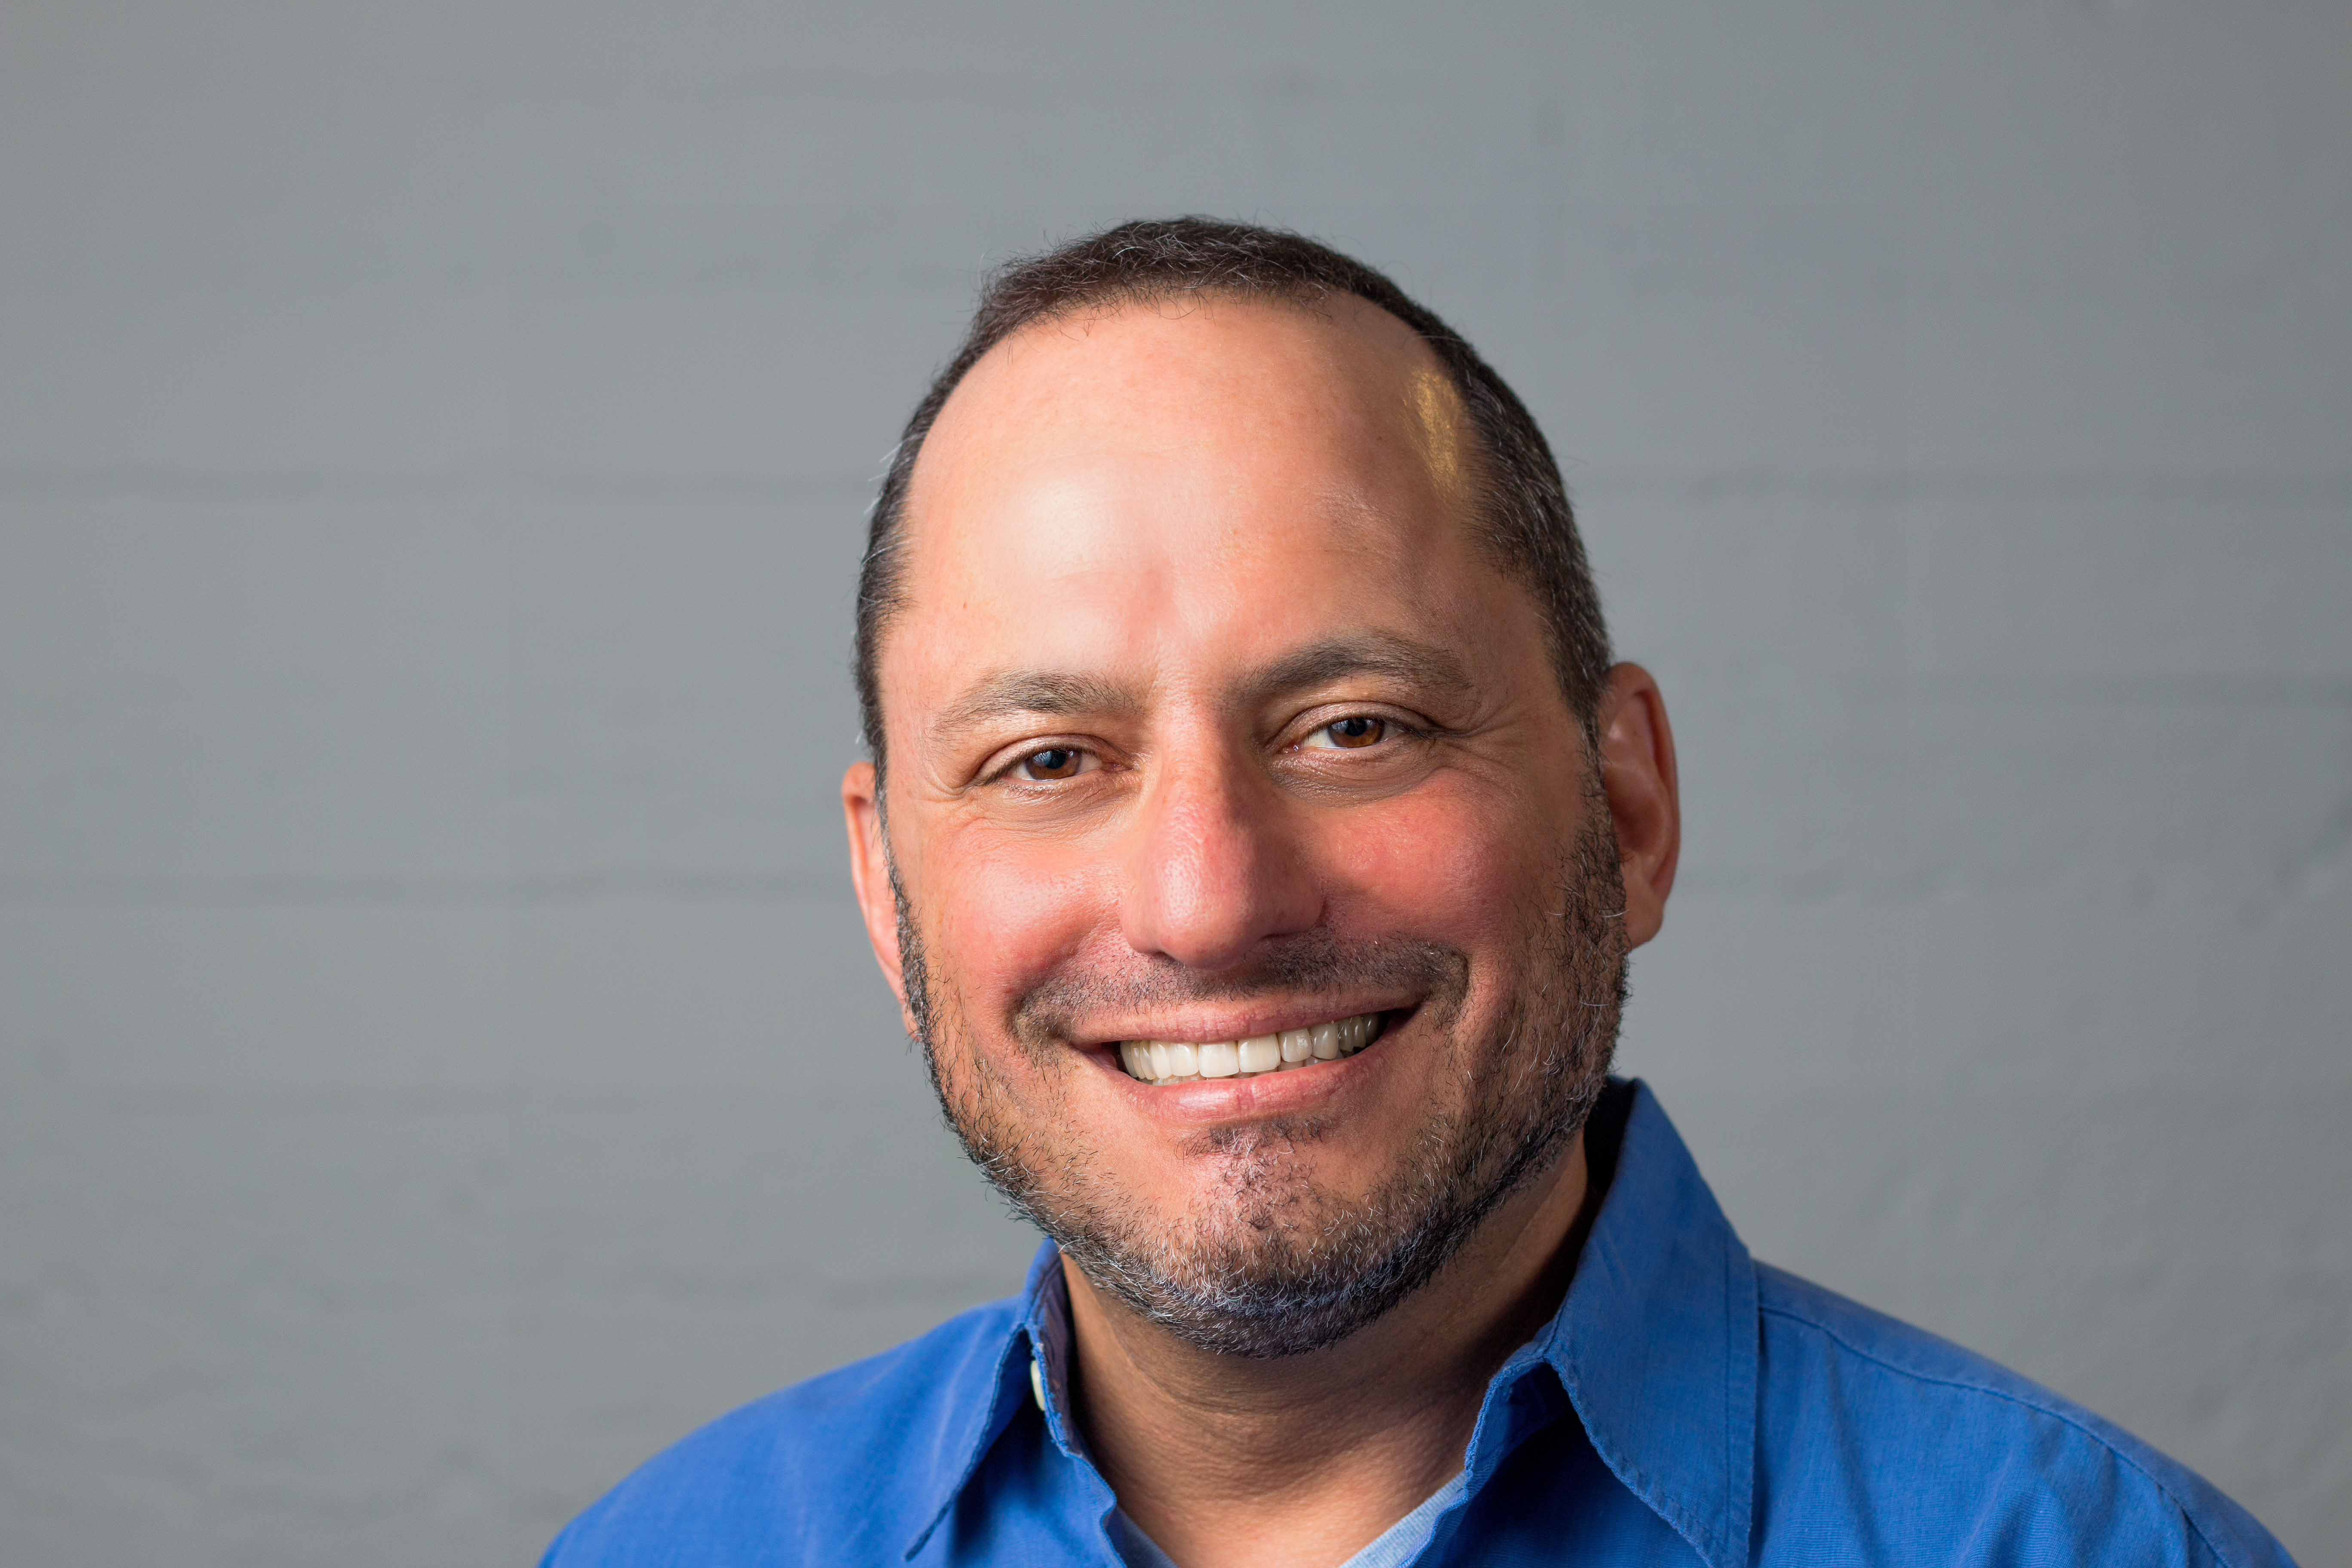
\includegraphics[width=0.19\textwidth]{figures/biography/Danny.jpg}
%   \hspace{-0.02in}
%   \vspace{-0.02in}
%   \end{center}
% \end{wrapfigure}
% \noindent\textbf{Dan Halperin} received his Ph.D. in Computer Science from Tel Aviv
% University. He then spent three years at the Computer Science
% Robotics Laboratory at Stanford University. In 1996 he joined the
% School of Computer Science at Tel Aviv University, where he is
% currently a full professor. Halperin's main field of research is
% Computational Geometry and its Applications. A major focus of his
% work has been in research and development of robust geometric
% software, principally as part of the CGAL project and library. The
% application areas he is interested in include robotics, automated
% manufacturing, algorithmic motion planning and 3D printing.
% http://acg.cs.tau.ac.il/danhalperin\\

%\begin{figure}[h]

%\begin{wrapfigure}{l}{0.25\textwidth}
%\begin{center}
%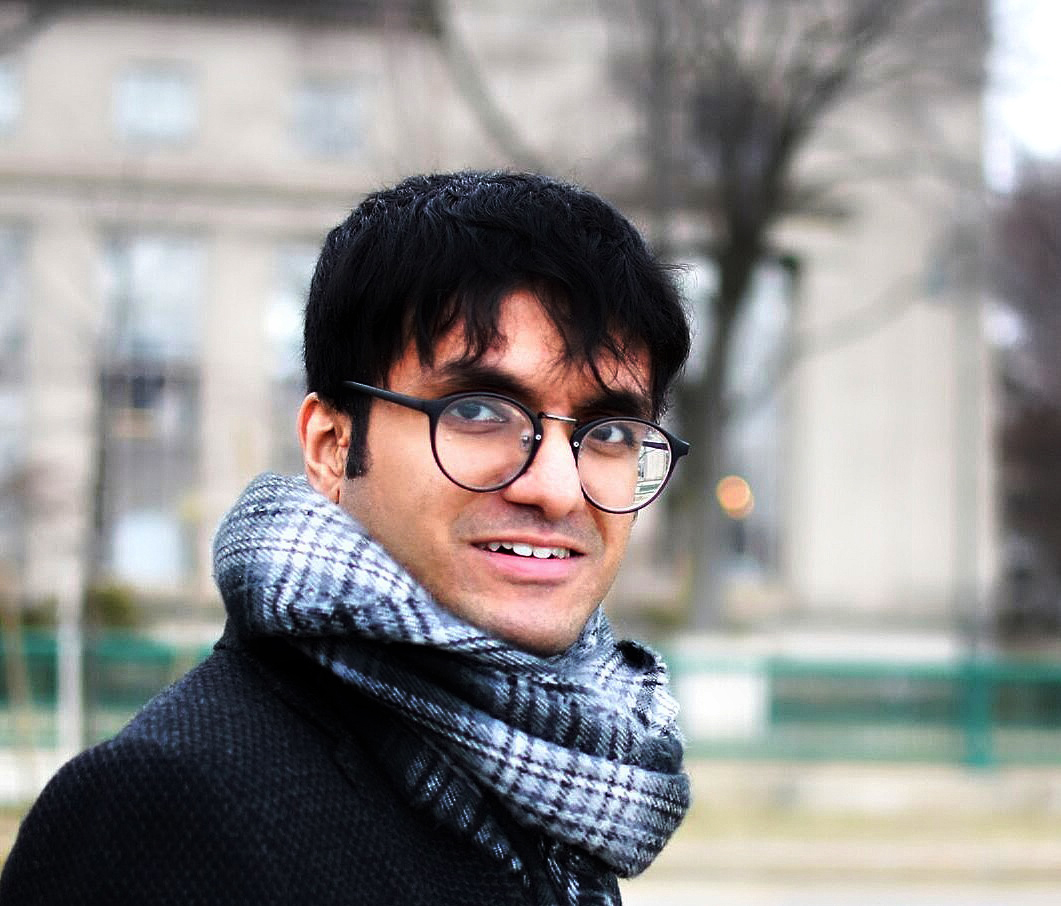
\includegraphics[width=0.24\textwidth]{figures/biography/rahul_shome.jpeg}
%\end{center}
%\end{wrapfigure} \par 
\vspace{0.3in}
\parpic{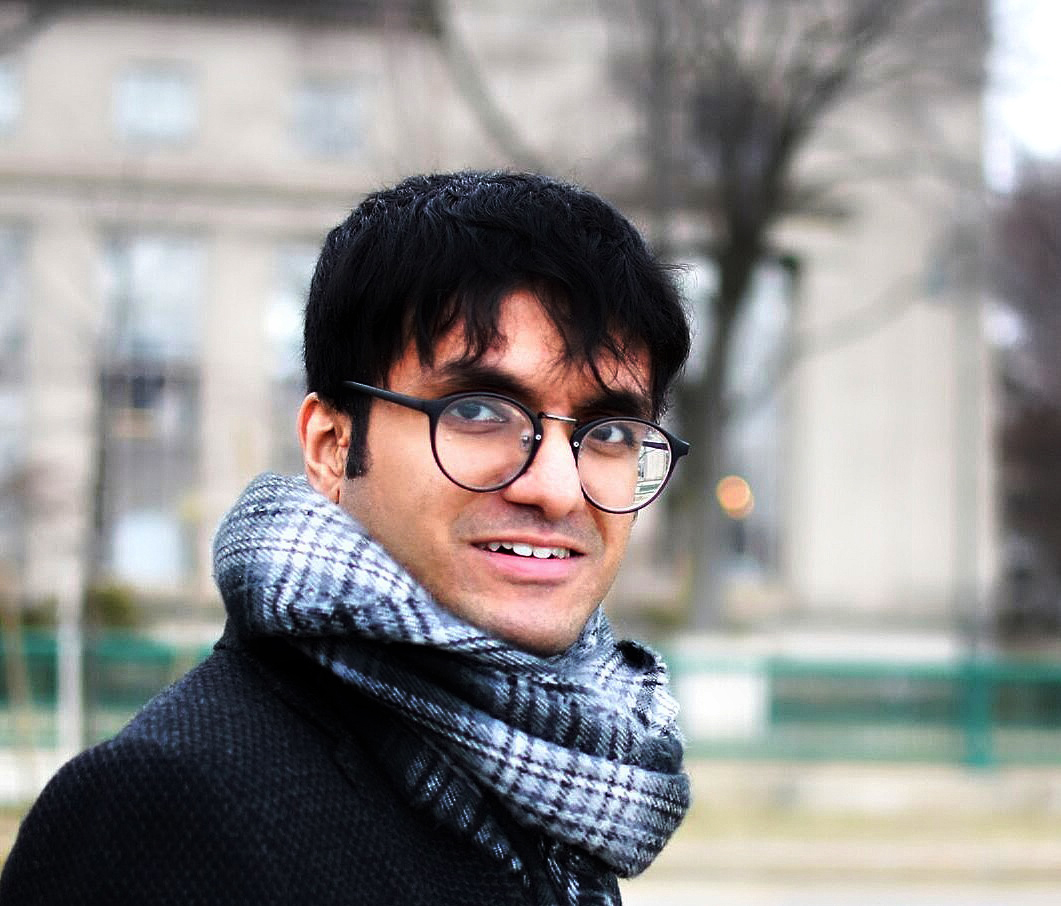
\includegraphics[width=0.2\textwidth]{figures/biography/rahul_shome.jpeg}}
\noindent {\bf Rahul Shome} is a Postdoctoral Research Associate at Kavraki Lab, Rice University, working with Prof. Lydia Kavraki. He attained his Ph.D. in Computer Science from Rutgers University where he worked with Prof. Kostas Bekris at the PRACSYS Lab. His research interests include motion
planning, manipulation, and task-and-motion planning with a special focus on practical real-world robotic solutions with strong theoretical guarantees. 

\vspace{0.2in}
%\begin{wrapfigure}{l}{0.2\textwidth}
%  \centering
  % \vspace{-0.02in}
%    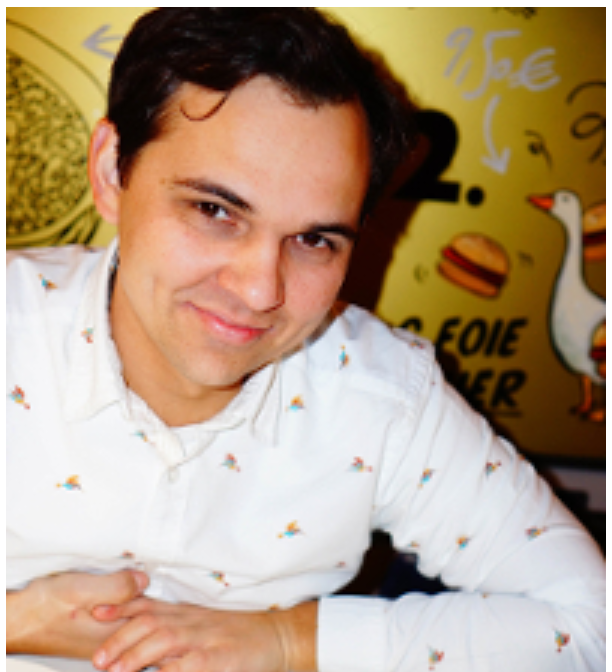
\includegraphics[width=0.19\textwidth]{figures/biography/kiril_solovey.PNG}
  % \hspace{-0.02in}
  % \vspace{-0.02in}
%\end{wrapfigure}

\parpic{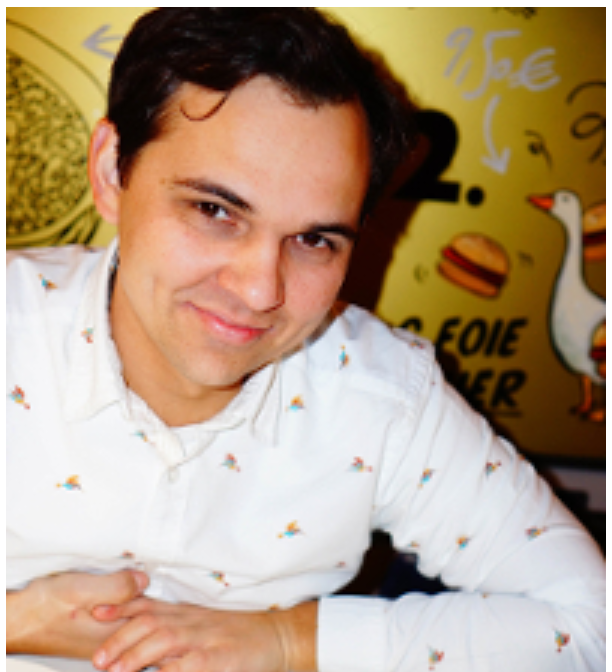
\includegraphics[width=0.2\textwidth]{figures/biography/kiril_solovey.PNG}}
\noindent {\bf Kiril Solovey} is a Postdoctoral Scholar at the Autonomous Systems Lab, Department of Aeronautics and Astronautics, Stanford University, hosted by Prof. Marco Pavone. His research focuses on algorithmic aspects of robotics. He is particularly interested in the design and analysis of techniques for robot motion planning, multi-robot systems, and autonomous mobility-on-demand. He is supported by the Fulbright Scholars Program. Prior to Stanford, He was a Ph.D. student at Tel Aviv University working with Prof. Dan Halperin in the Computational Geometry Lab. He was supported by the Clore Israel Foundation.

\vspace{0.2in}

\parpic{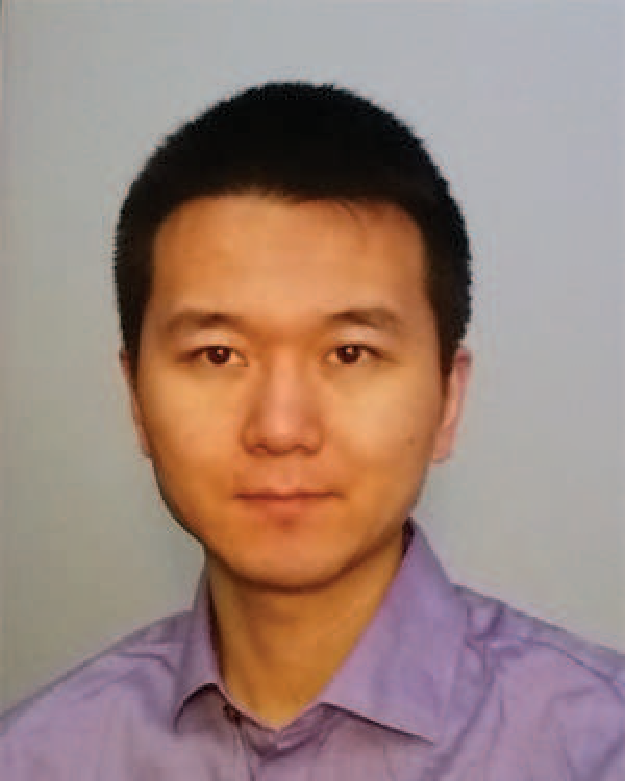
\includegraphics[width=0.2\textwidth]{figures/biography/yu-eps-converted-to.pdf}}
\noindent {\bf Jingjin Yu} is an Assistant Professor in the Department of Computer Science at Rutgers, the State University of New Jersey. He received his B.S. degree from the University of Science and Technology of China in 1998. He holds M.S. degrees in Chemistry (Univ. Chicago, 2000), Mathematics (Univ. Illinois at Chicago, 2001), and Computer Science (Univ. Illinois at Urbana-Champaign, 2010). He obtained his Ph.D. degree in Electrical and Computer Engineering from the University of Illinois at Urbana-Champaign in 2013, where he briefly stayed as a postdoctoral researcher. He was a postdoctoral researcher at the Massachusetts Institute of Technology from 2013 to 2015 with a joint appointment at Boston University from 2013 to 2014. He is broadly interested in the areas of robotics and control, focusing on issues related to computational complexity and the design of efficient algorithms with provable guarantees. He is a Siebel Scholar and a recipient of the NSF CAREER Award.

\vspace{0.2in}

\parpic{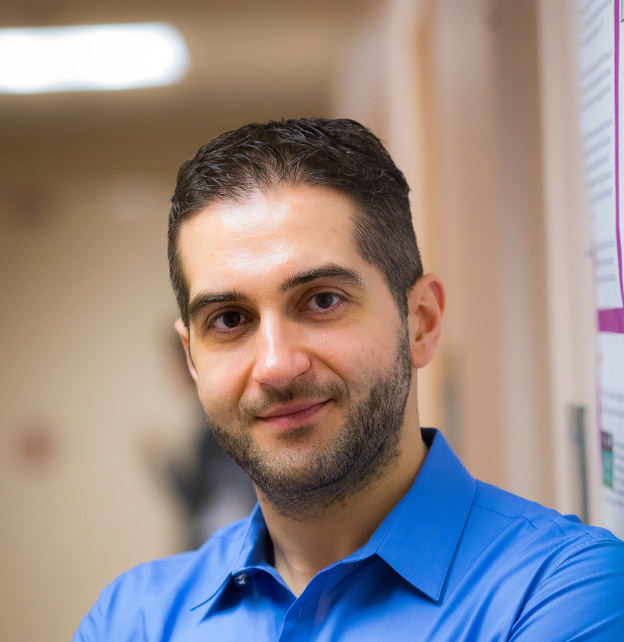
\includegraphics[width=0.2\textwidth]{figures/biography/kostas_bekris.jpg}}
\noindent {\bf Kostas Bekris} is an Associate Professor in the
Computer Science department of Rutgers University. He received his MS and PhD degrees in Computer Science from Rice University in 2004 and 2008 respectively. He was an Assistant
Professor at the Department of Computer Science and Engineering at the
University of Nevada, Reno from 2008 to 2012. He is the recipient of a
NASA Early Career Faculty award and his research has been supported by
NSF, NASA, DHS and the DoD. His research interests include planning
and coordination of robots, especially for systems with many degrees
of freedom and significant dynamics, as well as applications to
robot manipulation, planetary exploration, cyber-physical systems
and physically-realistic virtual agents. 

\vspace{0.2in}
\parpic{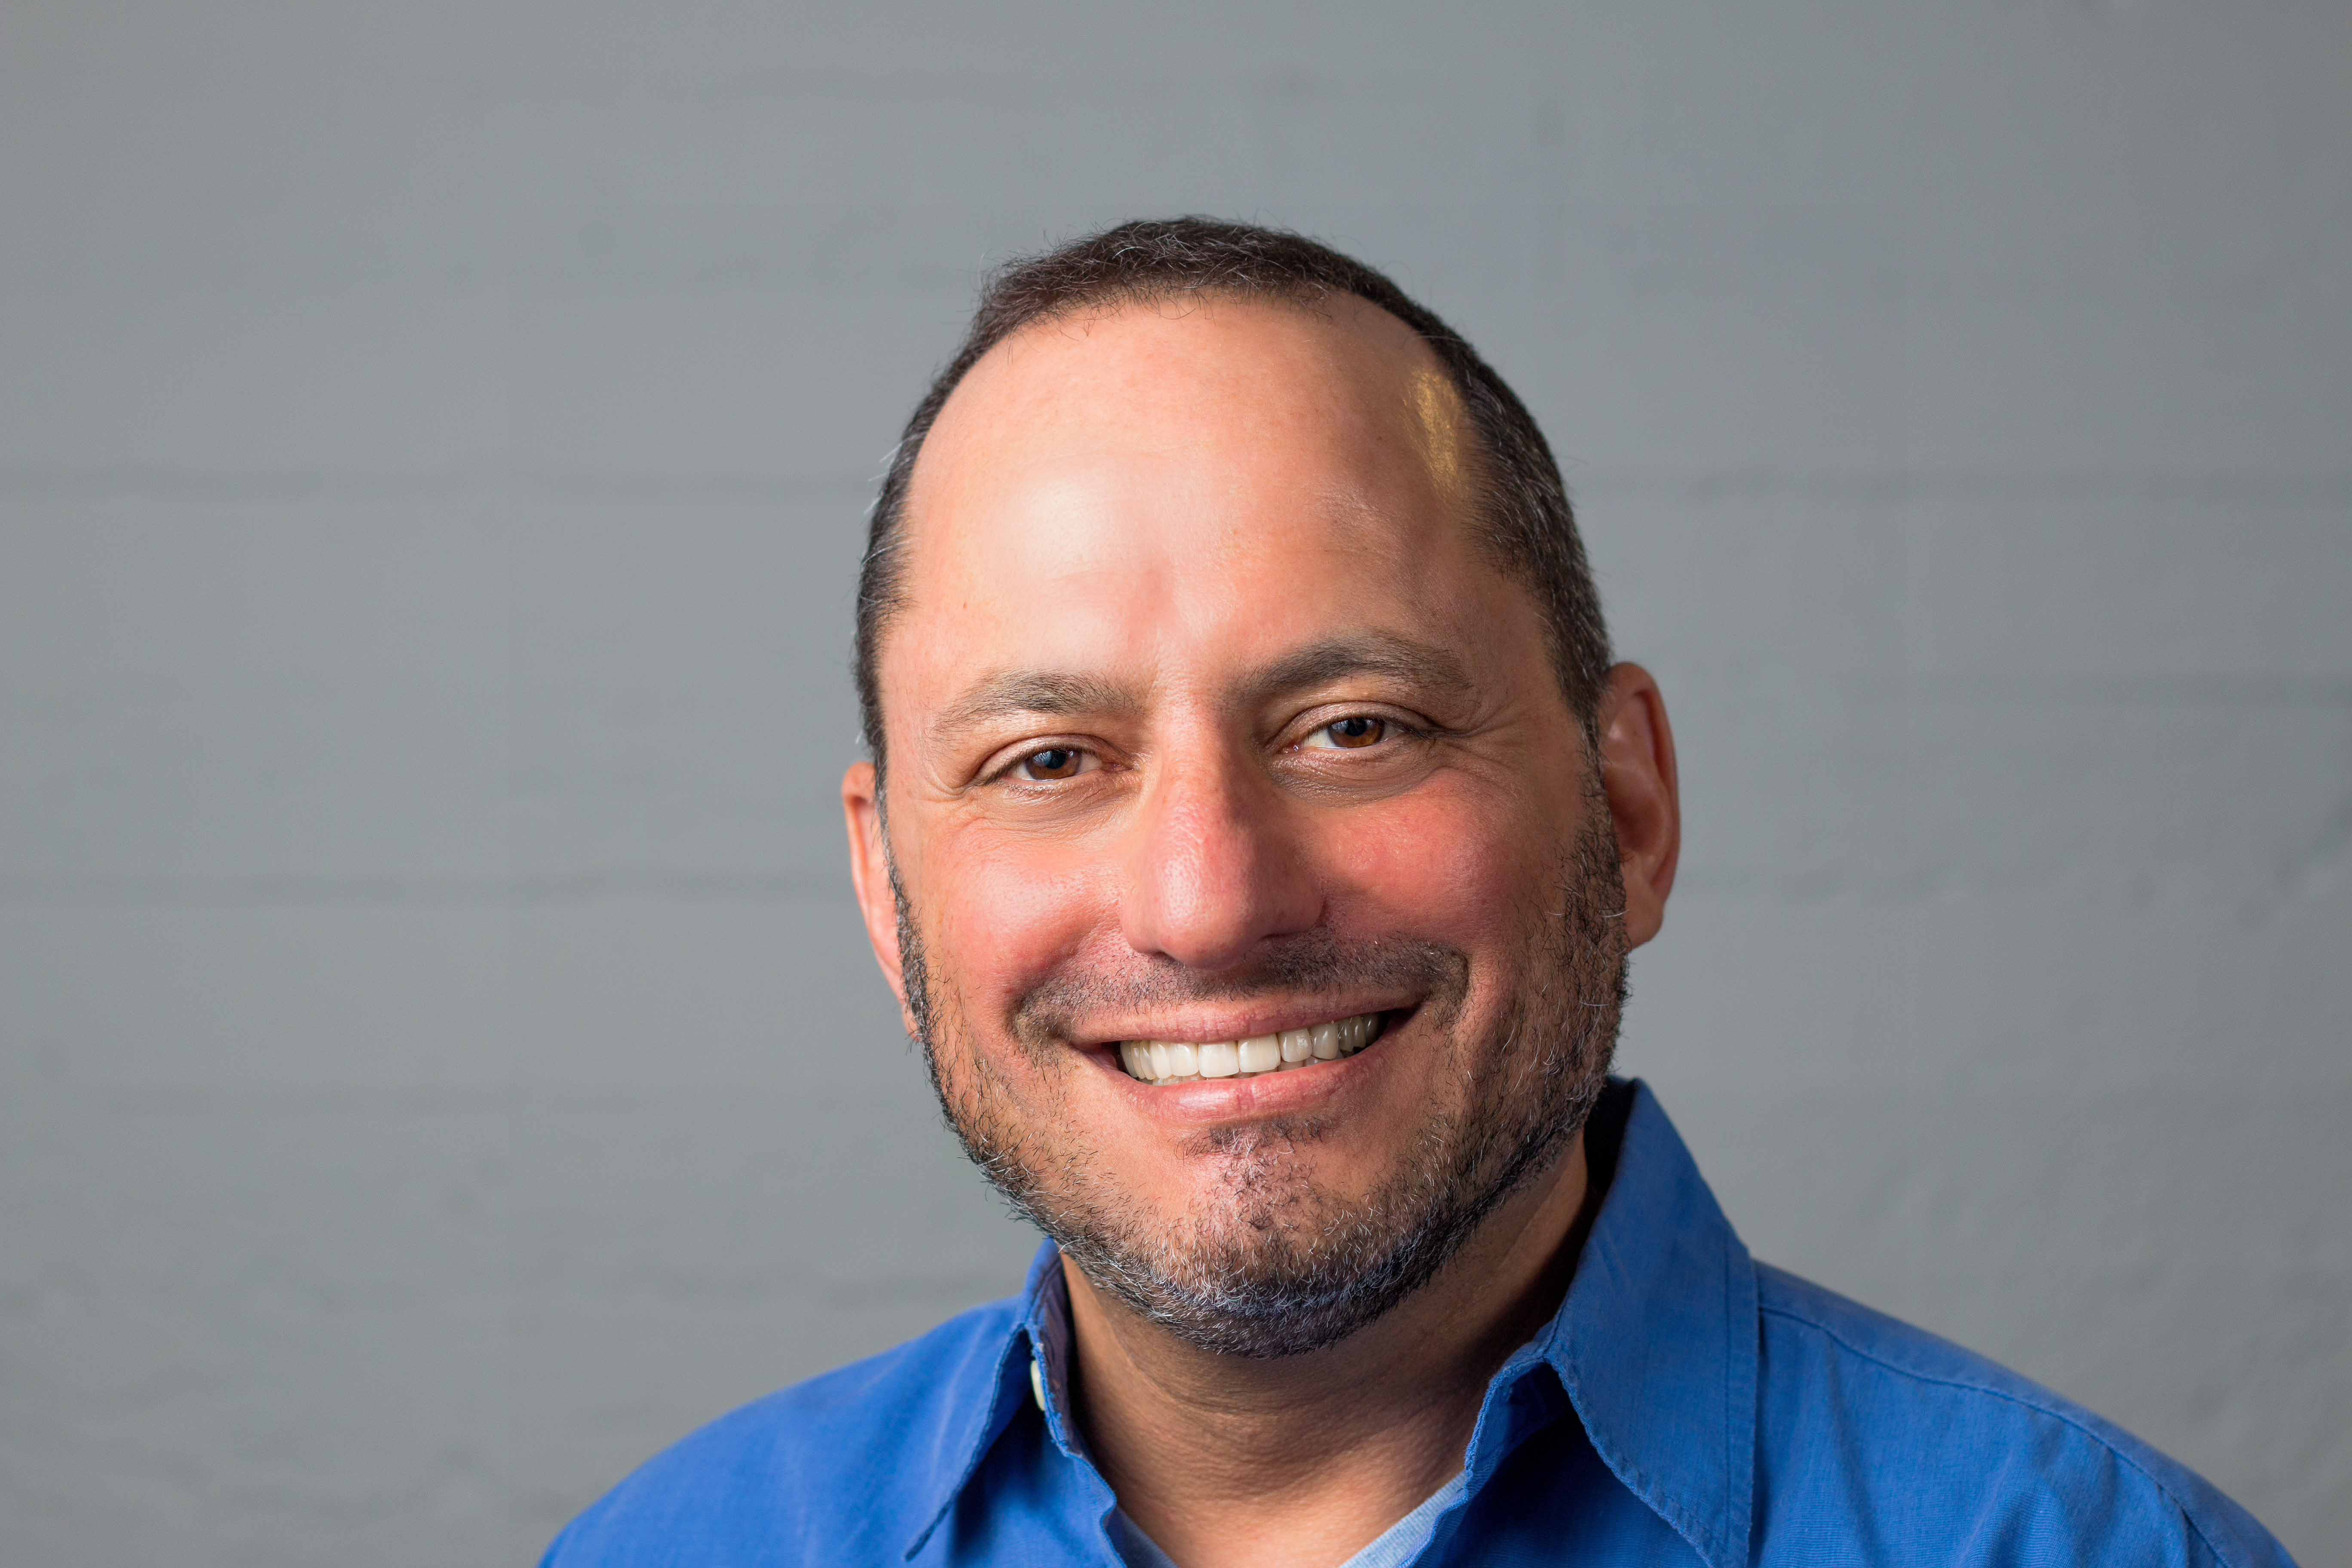
\includegraphics[width=0.2\textwidth]{figures/biography/Danny.jpg}}
\noindent {\bf Dan Halperin} received his Ph.D. in Computer Science from Tel Aviv University. He then spent three years at the Computer Science
Robotics Laboratory at Stanford University. In 1996 he joined the
School of Computer Science at Tel Aviv University, where he is
currently a full professor. Halperin's main field of research is
Computational Geometry and its Applications. A major focus of his
work has been in research and development of robust geometric
software, principally as part of the CGAL project and library. The
application areas he is interested in include robotics, automated
manufacturing, algorithmic motion planning and 3D printing.
http://acg.cs.tau.ac.il/danhalperin\\